\fancychapter{The work}

%TODO Nao posso posso aproveitar a architectura porque nao tem na a ver..
\begin{itemize}
  \item work on the inesc dataset
  \item work done on the crawller 
  \item work done on RubySOM 
  \item alterations on RubySOM to create Social version of SOM 
\end{itemize}

%% Sub multiple figures
%
%\begin{figure}[t]
%\centering
%\subfigure[caption for subfigure a]{\includegraphics[scale=0.65]{images/img1.eps}\label{chp3:img1}}
%\hspace*{0.5cm}
%\subfigure[caption for subfigure b]{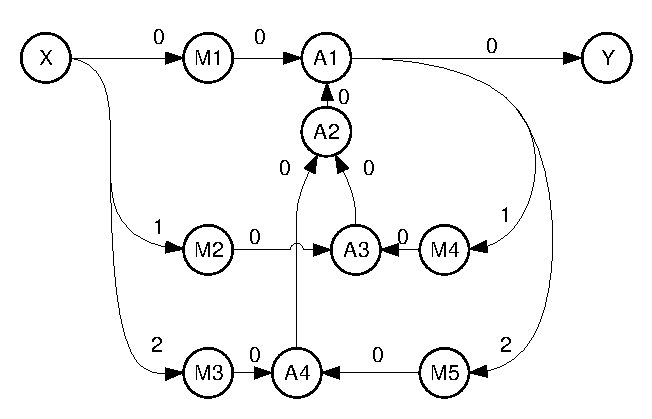
\includegraphics[scale=0.65]{images/img2.eps}\label{chp3:img2}}\\
%\caption{A figure example.}
%\label{fig:rmain figure}
%\end{figure}
%See the source code to see how to reference each of the subfigures \ref{chp3:img1} or \ref{chp3:img2}, or the main figure \ref{fig:rmain figure}.

%% how to add formulas
%There are several ways to define formulas (see the \textit{Short Math Guide for LaTeX} included in the package). The typical method is to use (see source code): 
%\begin{equation}
%a= b + c
%\end{equation}
%or
%\begin{align}
%c &= d \cdot e \nonumber\\
%d &= \mathbf{X}^{\mathsf{T}} \mathbf{Y}+ \gamma e^{2\pi}
%\label{chp3:eq1} 
%\end{align}
%or
%\begin{subequations}
%\begin{align}
%c &= d \cdot e \label{chp3:eq2:a} \\
%d &= \mathbf{X}^{\mathsf{T}} \mathbf{Y} + \gamma e^{2\pi}
%\label{chp3:eq2:b} 
%\end{align}
%\label{chp3:eq2} 
%\end{subequations}
%where $\mathbf{X}$ and $\mathbf{Y}$ are column vectors (you should always present the meaning of each parameter). The \textbf{AMS} packages allow to use the command \verb"\eqref" to cite equations such as \eqref{chp3:eq1},  \eqref{chp3:eq2:a},\eqref{chp3:eq2:b} or \eqref{chp3:eq2} (see source code).

\section{Summary}
An ending section summarizing the chapter is typically a good idea.

% Ensure that the next chapter starts in a odd page
\cleardoublepage
 
